
\documentclass[a4paper, 12pt]{article}
\usepackage{a4wide}
\usepackage {amsmath}
\usepackage{amssymb}
\usepackage {graphicx}
\usepackage[utf8]{inputenc} 
\usepackage[francais]{babel}
\usepackage{fancyhdr}
\usepackage{setspace}
\usepackage{fancyhdr}
\usepackage{lastpage}
\usepackage{extramarks}
\usepackage{chngpage}
\usepackage{soul}
\usepackage{algorithmicx} 
\usepackage{algpseudocode} 
\usepackage{multicol}
\usepackage[usenames,dvipsnames]{color}
\usepackage{graphicx,float,wrapfig}
\usepackage{ifthen}
\usepackage{listings}
\usepackage{courier}
\usepackage{esint}
\usepackage{bbm}
\usepackage{graphics}
\usepackage{graphicx}
\usepackage{subfig}
\usepackage{epsfig}
\usepackage{pgf,tikz}
\usetikzlibrary{arrows}
\usepackage{braket}
\usepackage{MnSymbol,wasysym}
\usepackage{marvosym}
\usepackage{dsfont}
\usepackage{stmaryrd}

\lhead{} 
\chead{} 
\rhead{\bfseries Modes propres} 
\lfoot{JC}
%\cfoot{} 
%\rfoot{\thepage}

% This is the color used for MATLAB comments below
\definecolor{MyDarkGreen}{rgb}{0.0,0.4,0.0}

% For faster processing, load Matlab syntax for listings
\lstloadlanguages{Matlab}%
\lstset{language=Matlab,                        % Use MATLAB
        frame=single,                           % Single frame around code
        basicstyle=\small\ttfamily,             % Use small true type font
        keywordstyle=[1]\color{Blue}\bf,        % MATLAB functions bold and blue
        keywordstyle=[2]\color{Purple},         % MATLAB function arguments purple
        keywordstyle=[3]\color{Blue}\underbar,  % User functions underlined and blue
        identifierstyle=,                       % Nothing special about identifiers
                                                % Comments small dark green courier
        commentstyle=\usefont{T1}{pcr}{m}{sl}\color{MyDarkGreen}\small,
        stringstyle=\color{Purple},             % Strings are purple
        showstringspaces=false,                 % Don't put marks in string spaces
        tabsize=5,                              % 5 spaces per tab
        %
        %%% Put standard MATLAB functions not included in the default
        %%% language here
        morekeywords={xlim,ylim,var,alpha,factorial,poissrnd,normpdf,normcdf},
        %
        %%% Put MATLAB function parameters here
        morekeywords=[2]{on, off, interp},
        %
        %%% Put user defined functions here
        morekeywords=[3]{FindESS, homework_example},
        %
        morecomment=[l][\color{Blue}]{...},     % Line continuation (...) like blue comment
        numbers=left,                           % Line numbers on left
        firstnumber=1,                          % Line numbers start with line 1
        numberstyle=\tiny\color{Blue},          % Line numbers are blue
        stepnumber=5                            % Line numbers go in steps of 5
        }

% Includes a MATLAB script.
% The first parameter is the label, which also is the name of the script
%   without the .m.
% The second parameter is the optional caption.
\newcommand{\matlabscript}[2]
  {\begin{itemize}\item[]\lstinputlisting[caption=#2,label=#1]{#1.m}\end{itemize}}

\pagestyle{fancy}

\begin{document}

\bibliographystyle{alpha}

\title{Modes propres de vibration d'une membrane}

%\author{Quentin Rafhay - Jean-Christophe Toussaint\\
%  Phelma\\
%\texttt{jean-christophe.toussaint@phelma.grenoble-inp.fr}
%}
%\date{\today}
\date{\vspace{-10ex}}
 
\maketitle

 
Le but de l'exercice est de caractériser les modes de vibration $u_k(x,y)$ selon Oz d'une membrane
rectangulaire de faible épaisseur. Dans la limite des faibles amplitudes de vibration, 
ils sont solutions de l'équation d'Helmholtz stationnaire :

\begin{equation}
\partial_x^2 \; u_k + \partial_y^2 \; u_k + k^2 \; u_k=0
\label{Helm}
\end{equation}

On considère que la membrane rectangulaire est fixée sur ses quatre cotés.


\section{Partie Mathématique}

La membrane de longueurs $L_x$ et $L_y$ selon les axes principaux est dicrétisée en différences finies
avec une grille comportant $N_x$ noeuds selon Ox et $N_y$ noeuds selon Oy. On note $\Delta x$ et
$\Delta y$ les pas de la grille.

\begin{enumerate} 
\item Donner les expressions de $\Delta x$ et $\Delta y$.
 \item  On numérote de manière unique les noeuds dans $\llbracket 0, N_x. N_y  \llbracket$. 
Montrer qu'un choix de numérotation possible est donné par la relation 
${\tt ind}(ix, iy)=iy*N_x+~ix$ où
$(ix, iy) \in \llbracket 0, N_x-1 \rrbracket \times \llbracket 0, N_y-1  \rrbracket$.
Comment parcourt-on la grille? Quelles sont
les coordonnées réelles $(x, y)$ d'un noeud de coordonnées entières $(ix, iy)$ en plaçant
{\bf l'origine des coordonnées en bas et à gauche}.
    
 \item Donner l'expression discrète en différences finies, de l'opérateur laplacien appliqué à $u(x, y)$ 
 en un point {\bf intérieur} $(x, y)$ de la grille rectangulaire, forme généralisé de celui unidimensionnel vu en cours. 

 {\it Indication} : faire un développement de Taylor de $u(x, y)$ à partir des premiers voisins.
On utilisera le développement limité suivant, pour une fonction à deux variables :
  \begin{equation}
 u(x+dx, y+dy) = u(x, y) + dx\; \partial_x u + dy\;  \partial_y u + \frac{1}{2} (dx\;  \partial_x + dy\; \partial_y)^2 \; u+
 \vartheta(dx, dy)^3
\end{equation}
où $(dx, dy)$ sont des déplacements infinitésimaux. Les dérivées partielles étant évaluées en $(x, y)$. 

Réponse : $$\Delta u = \frac{u(x+dx, y)+u(x-dx, y)-2u(x, y)}{dx^2}+\frac{u(x, y+dy)+u(x, y-dy)-2u(x, y)}{dy^2}$$

\item Montrer que l'on peut écrire l'équation  \eqref{Helm}  après discrétisation, sous la forme matricielle :
\begin{equation}
\sum_j K_{i, j} \; u_j = k^2 u_i = \lambda_k u_i
\label{HelmDis}
\end{equation}
Préciser la forme générale de la matrice K sans se soucier des bords.

\item On tient maintenant compte du déplacement nul des noeuds du bord.
Dans le cas d'une grille $4 \times 4$ de pas de maille $\Delta x$ et $\Delta y$ , donner
précisément le remplissage de $K$ avec l'expression des termes non-nuls. 
Dans la suite, on verra comment éliminer les degrés de liberté liés aux noeuds de dirichlet.
On admet que pour tout noeud ${i}$ du bord, on laisse vide la ligne  ${i}$ dans la matrice $K$.
Utiliser le patron de la matrice vide fournie en annexe.

\end{enumerate} 

\section{Modes propres avec conditions de dirichlet}

On présente ici une méthode générale pour calculer les modes propres en 
tenant compte des conditions de vibration nulle sur le bord .

En notant $N_d$ le nombre de noeuds où  la condition de dirichlet est imposée, 
le nombre de degrés de liberté se réduit alors à $N_{dof}=N-N_d$ et correspond 
ici au nombre de noeuds pouvant vibrer.

%On montre que la liste unique des noeuds de dirichlet peut générer sous matlab grâce
%au script suivant
%\matlabscript{dirnoeuds}{liste unique des noeuds de bord}

\subsection{Algorithme}
%L'algorithme consiste à former une liste $l_{dof}$ où le numéro de chaque noeud pouvant osciller,
%apparaît de façon unique. Sa
%taille est $N_{dof}=N-N_d$ et s'identifie, ici,  au nombre de degrés de liberté. \\

L'algorithme consiste à former une liste $l_{d}$ où apparaissent de 
manière unique les numéros des noeuds fixes du bord. 

On forme  ensuite une matrice de projection $P$ permettant de passer de l'espace des solutions à $N$ degrés de liberté (étude précédente) à celui restreint à $N_{dof}$ degrés de liberté.
Les dimensions de P sont $N_{dof} \times N$ (nombre de lignes $\times$ nombre de colonnes).

On initialise la matrice $P$ avec  la matrice identité ${\tt Id}(N)$
puis de supprimer toutes les lignes correspondant aux noeuds de dirichlet. Cette technique
est bien adaptée à Matlab : si $ld$ est la liste des noeuds de dirichlet sans doublon alors \\
$P={\tt Id}(N); \; P(ld, :)=[ \;];$\\

\begin{figure}[!h]
\centering
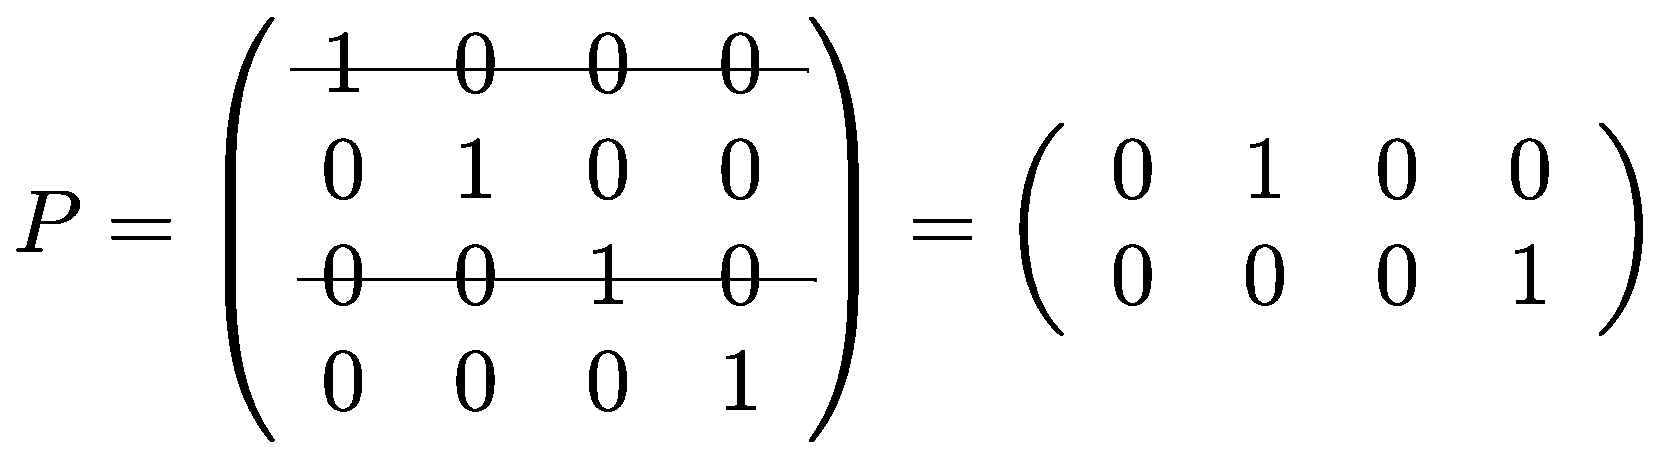
\includegraphics[scale=0.25]{matP.eps}
\caption{exemple de matrice $P$ avec $ld=[1, 3]$}
\label{matP}
\end{figure}

On construit ensuite $K_p$ qui est la matrice projetée de $K$ dans l'espace
solution à $N_ {dof}$ degrés de liberté: $K_p=P K P^t$ . \\

On résoud l'équation aux valeurs propres :
$P K P^t u_p= \lambda_p u_p$.
%grâce au script matlab suivant:
%\matlabscript{ritz2}{ritz2}

On obtient alors les valeurs propres $\lambda_p$ associées
aux vecteurs propres $u_p$. 


On reconstruit la solution dans l'espace à $N$ noeuds en appliquant $u=P^t u_p$. 
Elle vérifie automatiquement, $u(i)=0$ pour tout noeud $i$ de dirichlet.
 
%\subsection{Phase de programmation et de simulation}
  
\section{Mise en application}

On vous fournit un embryon de programme {\tt numpy\_modes\_membrane.py}  à compléter,
utilisant une structure de
données {\tt fdm} pour stocker tous les paramètres de la simulation.

\begin{enumerate} 

\item Compléter la fonction  {\tt \_\_dirichlet} permettant de construire la liste $ld$ 
des noeuds du bord où sont appliquées la conditions de dirichlet.
On rappelle que
l'instruction {\tt ld.append(e)} permet d'insérer l'élément e dans la liste ld. 
Utiliser sous Numpy, la fonction {\tt ld=numpy.unique(ld)} pour éliminer tout doublon dans la liste {\tt ld}.

% \matlabscript{founddir}{test dirichlet}

\item Compléter la fonction  {\tt \_\_build\_K} permettant de remplir la matrice $K$ pour une grille
de taille $N_x$.  On rappelle que toute ligne $n$ de $K$ correspondant à un noeud
de dirichlet n'est pas remplie. \\
Pour tester l'appartenance d'un noeud $n$ dans la liste {\tt ld}, on utilisera l'expression booléenne
 {\tt n in ld}. 

\item Compléter  la fonction  {\tt solve} permettant de calculer la $n^{eme}$ plus petite valeur propre
en module ainsi que le mode propre associé. On utilisera la fonction Numpy {\tt eig} 

\item Pour un système rectangulaire de taille $L_x=2m$ et $L_y=1m$, déterminer les 4 premiers modes de basse énergie et comparer à la solution analytique de l'équation d'Helmholtz \eqref{Helm}. 
{\it Indication} : chercher des solutions de la forme $\sin(k_x x).\sin(k_y y)$.
Reporter les valeurs propres et les contours des modes associés sur votre copie.

\item Faire de même pour $L_x=1m$ et $L_y=1m$, expliquer pourquoi les modes d'ordre 2 et 3
semblent différents de ceux calculés analytiquement.
{\it Indication} : regarder la dégénerescence des valeurs propres.

\end{enumerate} 



\section{Annexe - Nom .......................... Prénom ....................}

\begin{center}
   \begin{tabular}{| c | c | c | c | c | c | c | c | c | c | c | c | c | c | c | c | c | }
     \hline
     & 1. & 2. & 3. & 4. & 5. & 6. & 7. & 8. & 9. & 10 & 11 & 12 & 13 & 14 & 15 & 16\\ \hline
     1 &  &   &   &   &   &   &   &   &  &  &  &  &  &  &  &\\ \hline
     2 &  &   &   &   &   &   &   &   &  &  &  &  &  &  &  &\\ \hline
     3 &  &   &   &   &   &   &   &   &  &  &  &  &  &  &  &\\ \hline
     4 &  &   &   &   &   &   &   &   &  &  &  &  &  &  &  &\\ \hline
     5 &  &   &   &   &   &   &   &   &  &  &  &  &  &  &  &\\ \hline
     6 &  &   &   &   &   &   &   &   &  &  &  &  &  &  &  &\\ \hline
     7 &  &   &   &   &   &   &   &   &  &  &  &  &  &  &  &\\ \hline
     8 &  &   &   &   &   &   &   &   &  &  &  &  &  &  &  &\\ \hline     
     9 &  &   &   &   &   &   &   &   &  &  &  &  &  &  &  &\\ \hline
   10 &  &   &   &   &   &   &   &   &  &  &  &  &  &  &  &\\ \hline    
   11 &  &   &   &   &   &   &   &   &  &  &  &  &  &  &  &\\ \hline    
   12 &  &   &   &   &   &   &   &   &  &  &  &  &  &  &  &\\ \hline    
   13 &  &   &   &   &   &   &   &   &  &  &  &  &  &  &  &\\ \hline    
   14 &  &   &   &   &   &   &   &   &  &  &  &  &  &  &  &\\ \hline    
   15 &  &   &   &   &   &   &   &   &  &  &  &  &  &  &  &\\ \hline    
   16 &  &   &   &   &   &   &   &   &  &  &  &  &  &  &  &\\ \hline    
     \hline
   \end{tabular}
 \end{center}
\hspace{20pt}
\begin{center}
   \begin{tabular}{| c | c | c | c | c | c | c | c | c | c | c | c | c | c | c | c | c | }
     \hline
     & 1. & 2. & 3. & 4. & 5. & 6. & 7. & 8. & 9. & 10 & 11 & 12 & 13 & 14 & 15 & 16\\ \hline
     1 &  &   &   &   &   &   &   &   &  &  &  &  &  &  &  &\\ \hline
     2 &  &   &   &   &   &   &   &   &  &  &  &  &  &  &  &\\ \hline
     3 &  &   &   &   &   &   &   &   &  &  &  &  &  &  &  &\\ \hline
     4 &  &   &   &   &   &   &   &   &  &  &  &  &  &  &  &\\ \hline
     5 &  &   &   &   &   &   &   &   &  &  &  &  &  &  &  &\\ \hline
     6 &  &   &   &   &   &   &   &   &  &  &  &  &  &  &  &\\ \hline
     7 &  &   &   &   &   &   &   &   &  &  &  &  &  &  &  &\\ \hline
     8 &  &   &   &   &   &   &   &   &  &  &  &  &  &  &  &\\ \hline     
     9 &  &   &   &   &   &   &   &   &  &  &  &  &  &  &  &\\ \hline
   10 &  &   &   &   &   &   &   &   &  &  &  &  &  &  &  &\\ \hline    
   11 &  &   &   &   &   &   &   &   &  &  &  &  &  &  &  &\\ \hline    
   12 &  &   &   &   &   &   &   &   &  &  &  &  &  &  &  &\\ \hline    
   13 &  &   &   &   &   &   &   &   &  &  &  &  &  &  &  &\\ \hline    
   14 &  &   &   &   &   &   &   &   &  &  &  &  &  &  &  &\\ \hline    
   15 &  &   &   &   &   &   &   &   &  &  &  &  &  &  &  &\\ \hline    
   16 &  &   &   &   &   &   &   &   &  &  &  &  &  &  &  &\\ \hline    
     \hline
   \end{tabular}
 \end{center}
 
 \newpage
 
% \matlabscript{FDhelmM1etud}{Embryon de programme}
\end{document}

